% Hi! We're member of IRIS-HEP and the Scikit-HEP community project, where we are building
% a Pythonic data analysis ecosystem for HEP community.
% IRIS-HEP does lots of things from data delivery, to cyberinfrastructure, and supporting the
% development of existing software tools, and has been a community center for fostering Scikit-HEP
% development.
% A shared goal is that we want to empower analysts at the LHC and beyond with modern data science stacks
% and build powerful libraries that allow for analysts to build expressive analysis workflows.
% \begin{frame}{Hello from IRIS-HEP and Scikit-HEP!}
%   \begin{columns}
%     \column{0.6\textwidth}
%     \Large
%     % \begin{itemize}
%     \begin{itemize}\setlength{\itemsep}{0.5 cm}
%       \item We're members of the \href{https://iris-hep.org/}{Institute for Research and Innovation in Software for High Energy Physics (IRIS-HEP)} and the \href{https://scikit-hep.org/}{Scikit-HEP} community project developing a Pythonic data analysis ecosystem for HEP
%       \item Goals: Empower analysts with modern data science stacks and provide powerful libraries for building expressive workflows
%     \end{itemize}
% %
%     \column{0.4\textwidth}
%     \begin{figure}
%         \begin{center}
%             \href{https://iris-hep.org/}{
\includegraphics[width=0.9\linewidth]{iris-hep-logo-long.pdf}}
%             \href{https://scikit-hep.org/}{
\includegraphics[width=0.8\linewidth]{scikit-hep-logo.pdf}}
%         \end{center}
%     \end{figure}
%   \end{columns}
% \end{frame}

% \begin{frame}{Built with intentionality and interoperability}
%   \begin{columns}
%     \column{0.45\textwidth}
%     \begin{enumerate}\setlength{\itemsep}{0.5 cm}
%       \item[5] HEP-specific UI applications or packaged algorithms
%       \item[4] HEP-specific for common problems
%       \item[3] HEP-specific, foundational
%       \item[2] needed to create, but not really HEP-specific
%       \item[1] non-HEP software we depend on
%     \end{enumerate}
% %
%     \column{0.55\textwidth}
%     \begin{figure}
%         \begin{center}
%             \href{https://indico.cern.ch/event/1140031/}{\includegraphics[width=\linewidth]{shells-hep.pdf}}
%         \end{center}
%     \end{figure}
%   \end{columns}
% \end{frame}

\begin{frame}{Analysis Systems Team}
  \begin{columns}
    \column{0.4\textwidth}
    % \Large
    % \begin{itemize}
    \begin{itemize}\setlength{\itemsep}{0.1 cm}
      \item Wisconsin-Madison
      \begin{itemize}
        \item Kyle, Alex, Matthew
      \end{itemize}
      \item Washington
      \begin{itemize}
        \item Gordon, Mason, Tal
      \end{itemize}
      \item Princeton
      \begin{itemize}
        \item Jim, Henry, Ianna
      \end{itemize}
      \item University of Cincinnati
      \begin{itemize}
        \item Mike, Thomas
      \end{itemize}
      \item Illinois
      \begin{itemize}
        \item Mark, Ben
      \end{itemize}
      \item NYU
      \begin{itemize}
        \item Irina
      \end{itemize}
      \item University of Nebraska-Lincoln
      \begin{itemize}
        \item Oksana
      \end{itemize}
    \end{itemize}
%
    \column{0.6\textwidth}
    \begin{figure}
        \begin{center}
            \href{https://iris-hep.org/as.html}{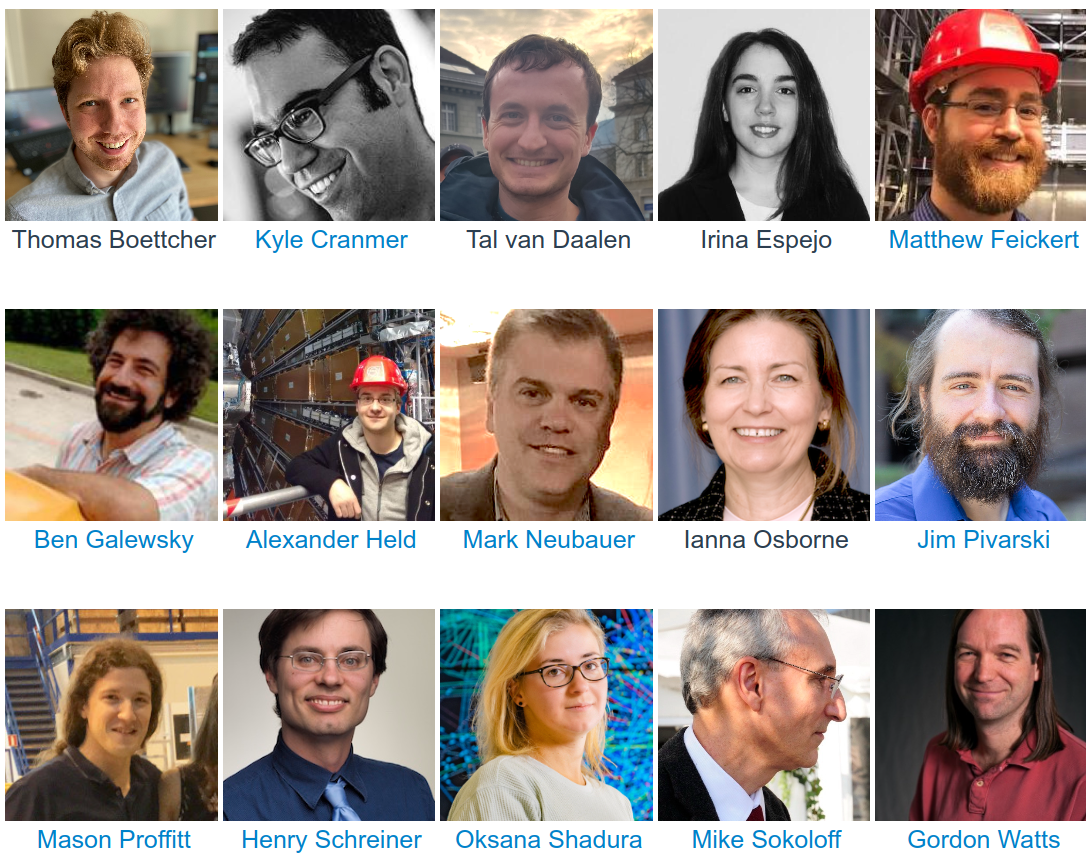
\includegraphics[width=\linewidth]{analysis-systems-team.png}}
        \end{center}
    \end{figure}
  \end{columns}
\end{frame}

\begin{frame}{Analysis Systems Projects}
  \begin{columns}
    \column{0.4\textwidth}
    % \begin{itemize}
    \begin{itemize}\setlength{\itemsep}{0.25 cm}
      \item Analysis Systems are connected to analysis use cases
      \item Systems are composed of components
      \item Large number of these projects refer to these componetns
      \begin{itemize}
        \item Many projects include people beyond IRIS-HEP directly
      \end{itemize}
      \item Milestones and activities are mainly oriented towards integration, evaluation, with a global overview of the vertical
    \end{itemize}
%
    \column{0.6\textwidth}
    \begin{columns}
      \begin{column}{0.5\textwidth}
        \begin{figure}
          \begin{center}
            \href{https://iris-hep.org/as.html}{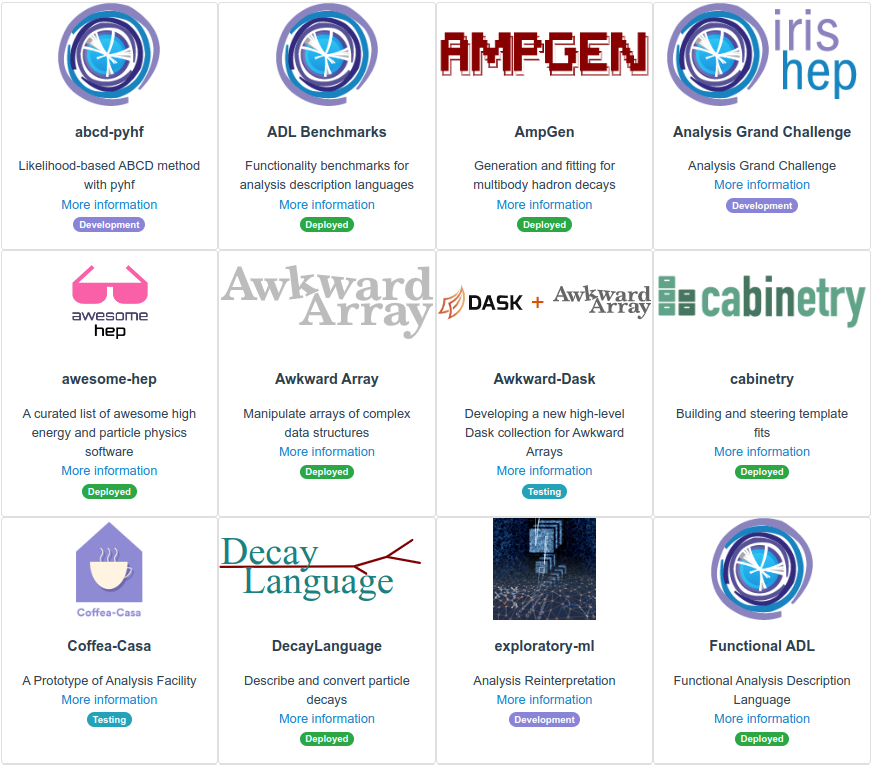
\includegraphics[width=\linewidth]{as_projects_1.png}}
          \end{center}
        \end{figure}
      \end{column}
      \begin{column}{0.5\textwidth}
        \begin{figure}
          \begin{center}
            \href{https://iris-hep.org/as.html}{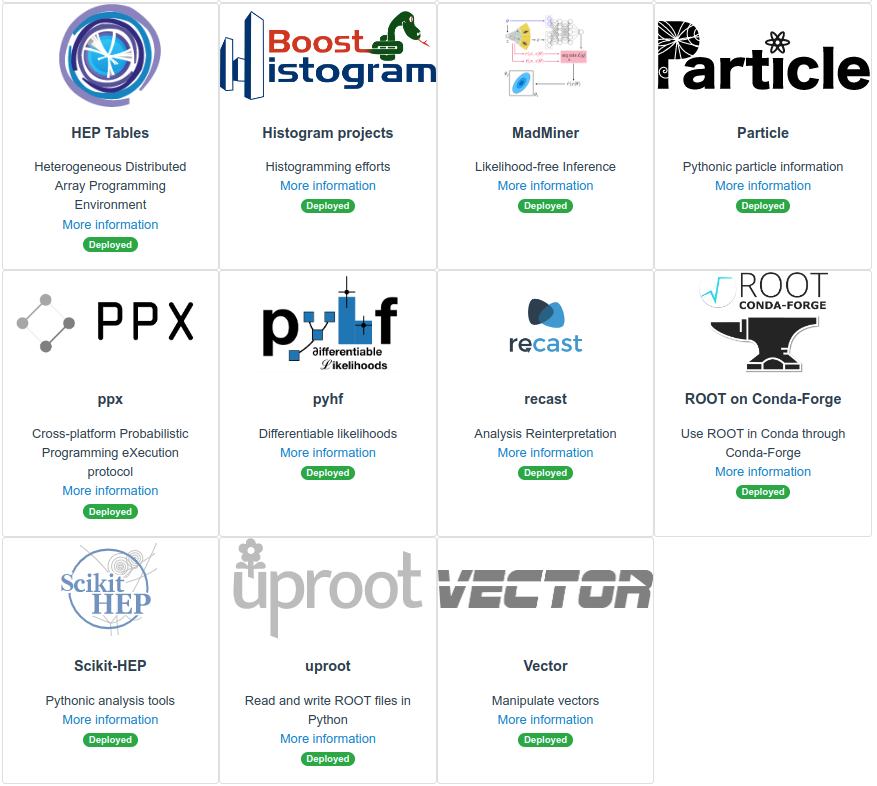
\includegraphics[width=\linewidth]{as_projects_2.png}}
          \end{center}
        \end{figure}
      \end{column}
    \end{columns}
    \begin{center}
      Analysis Systems Projects
    \end{center}
  \end{columns}
\end{frame}

\begin{frame}
  \frametitle{Analysis Systems Pipeline}

  \begin{itemize}
    \item Show the pipeline and the role that the project play in it
  \end{itemize}

\end{frame}

\begin{frame}
  \frametitle{Analysis Systems Goals}

  \begin{itemize}
    \item Lay out what the actual project goals are and where we're going here
    \item Compare to the requirements that we've agreed to
  \end{itemize}

\end{frame}

\begin{frame}
  \frametitle{Analysis Systems Project Progress}

  \begin{itemize}
    \item Highlight some project wins
    \item pyhf, cabinetry, awkward
  \end{itemize}

\end{frame}

\begin{frame}
  \frametitle{Analysis Systems Project Progress: Awkward}

  \begin{itemize}
    \item awkward
  \end{itemize}

\end{frame}

\begin{frame}
  \frametitle{Analysis Systems Project Progress: hist}

  \begin{itemize}
    \item hist
    \item Adoption in coffea
  \end{itemize}

\end{frame}

\begin{frame}
  \frametitle{Analysis Systems Project Progress: pyhf}

  \begin{itemize}
    \item pyhf
    \item probability model publishing
    \item Highlight wins in HSF with HEPData
  \end{itemize}

\end{frame}

\begin{frame}
  \frametitle{Analysis Systems Project Progress: cabinetry}

  \begin{itemize}
    \item cabinetry
    \item Analysis Grand Challenge work
  \end{itemize}

\end{frame}

\begin{frame}
  \frametitle{Analysis Systems Project Progress: Scikit-HEP}

  \begin{itemize}
    \item Continued growth
    \item PyHEP conferences ongoing
    \item Invitations from Scientific Python to get more invovled in borader community
  \end{itemize}

\end{frame}

\begin{frame}
  \frametitle{Analysis Systems Project Fellows}

  \begin{itemize}
    \item Quick highlight of fellow projects
    \item https://iris-hep.org/as.html
  \end{itemize}

\end{frame}
